%%% In this section, you will describe all of the various artifacts that you will generate and maintain during the project life cycle. Describe the purpose of each item below, how the content will be generated, where it will be stored, how often it will be updated, etc. Replace the default text for each section with your own description. Reword this paragraph as appropriate.

\subsection{Major Documentation Deliverables}
These deliverables are major grade components of the course. Completing these documents should generally be the sprint goal during the applicable sprint period. Remove this paragraph from your draft, but leave the heading.

\subsubsection{Project Charter}
Describe how this document will be maintained and updated (how often, under what circumstances, etc.). When will the initial version be delivered? When will the final version be delivered?

\subsubsection{System Requirements Specification}
This documnet will be updated anytime a new portion is added to the project. It will also be updates if there is a portion of the system that is found faulty or not feasible to work with. The intial version will be delievered along with the first charter report while the final version will be delievered when the design of the system has been concluded on and no changes need to be made.

\subsubsection{Architectural Design Specification}
This documnet will be updated anytime a new portion is added to the project. It will also be updates if there is a portion of the system that is found faulty or not feasible to work with. The intial version will be delievered along with the first charter report while the final version will be delievered when the design of the system has been concluded on and no changes need to be made.

\subsubsection{Detailed Design Specification}
This documnet will be updated anytime a new portion is added to the project. It will also be updates if there is a portion of the system that is found faulty or not feasible to work with. The new chnages will be described in detail showing what was removed or what was added in the design. The intial version will be delievered along with the first charter report while the final version will be delievered when the design of the system has been concluded on and no changes need to be made.

\subsection{Recurring Sprint Items}
The following items will be documented and maintained during each individual sprint. Remove this paragraph from your draft, but leave the heading.

\subsubsection{Product Backlog}
Team members will meet to determine requirements and break them down into features, which will be added to the backlog. Team members will determine the priority of each feature with a group vote, giving the most weight to items that progress development. The backlog will be a Google workbook document that can be edited and tracked by all team members.

\subsubsection{Sprint Planning}
At the end of one sprint there will be a meeting to discuss the next sprint. The backlog will be updated and tasks for each feature will be assigned. There will be 4 sprints, each lasting 3 weeks.

\subsubsection{Sprint Goal}
The team as a whole will determine the end goal of each sprint during the sprint planing meeting. The professor will be consulted periodically through the process via email and in-person communication. 

\subsubsection{Sprint Backlog}
The team as a whole will determine which backlog items are implemented into a sprint and when. The backlog will be a Google workbook document that can be edited and tracked by all team members.

\subsubsection{Task Breakdown}
The team will assign tasks during the sprint planing meeting. Team members can volunteer for tasks, or tasks can be assigned based on skill set. Task will be equally distributed across all members. Each team member will be responsible for tracking and recording the time spent on their assigned tasks. 

\subsubsection{Sprint Burn Down Charts}
Team members will alternate being scrum master. The scrum master will be responsible for monitoring the backlog. The backlog will generate a burn chart based on the data input into the table. Each team member will have access to update the backlog with the amount of time spent on each task. When this value is updated the burn chart will update the graph.

\begin{figure}[h!]
    \centering
    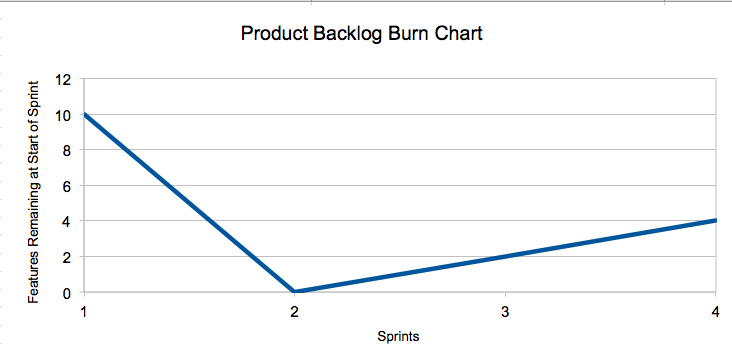
\includegraphics[width=0.5\textwidth]{images/burn_down_chart_example}
    \caption{Example sprint burn down chart}
\end{figure}

\subsubsection{Sprint Retrospective}
The sprint retrospective will take place at a team meeting. It will occur after every sprint has passed . The group will document what worked and should be maintained, what needs to improve and also resolve any conflict that arises in the just concluded sprint. It will be due about a week after the meeting has been held.

\subsubsection{Individual Status Reports}
Each member would report on any task that has been asssigned to them to work on. It will be reported anytime there is a new task assigned and also when the report needs to be turned in. Every item assigned to each individual relating to the building of the project is considered a key item and should be added in the report.

\subsubsection{Engineering Notebooks}
The engineering notebook will be updated anytime work is done on the project. Therefore each member would always enter any part of the project they are working on. The minimum amount of pages as of now should be 1 page. Every section of the project assigned by the group is considered an interval so each interval is till the that section is finished. At least two other team members will sign the engineering notebooks as witnesses for each page.

\subsection{Closeout Materials}
The following materials, in addition to major documentation deliverables, will be provided to the customer upon project closeout. Remove this paragraph from your draft, but leave the heading.

\subsubsection{System Prototype}
What will be included in the final system prototype? How and when will this be demonstrated? Will there be a Prototype Acceptance Test (PAT) with your customer? Will anything be demonstrated off-site? If so, will there be a Field Acceptance Test (FAT)?

\subsubsection{Project Poster}
What will be included on the poster, what will be the final dimensions, and when will it be delivered?

\subsubsection{Web Page}
What will be included on the project web page? Will it be accessible to the public? When will this be delivered? Will it be updated throughout the project, or just provided at closeout (at a minimum, you need to provide a simple web page at the end).

\subsubsection{Demo Video}
What will be shown in the demo video(s)? Will you include a B-reel footage for future video cuts? Approximately how long will the video(s) be, and what topics will be covered?

\subsubsection{Source Code}
How will your source code be maintained? What version control system will you adopt? Will source code be provided to the customer, or binaries only? If source code is provided, how will it be turned over to the customer? Will the project be open sourced to the general public? If so, what are the license terms (GNU, GPL, MIT, etc.). Where will the license terms be listed (in each source file, in a single readme file, etc.).

\subsubsection{Source Code Documentation}
What documentation standards will be employed? Will you use tools to generate the documentation (Doxygen, Javadocs, etc.). In what format will the final documentation be provided (PDF, browsable HTML, etc.)?

\subsubsection{Hardware Schematics}
Will you be creating printed circuit boards (PCBs) or wiring components together? If so, list each applicable schematic and what sort of data it will contain (PCB layout, wiring diagram, etc.). If your project is purely software, omit this section.

\subsubsection{CAD files}
Will the project involve any mechanical design, such as 3D printed or laser-cut parts? If so, what software will you use to generate the files and what file formats will you provide in your closeout materials (STL, STEP, OBJ, etc.). If your project is purely software, omit this section.

\subsubsection{Installation Scripts}
How will the customer deploy software to new installations? Will you provide installation scripts, install programs, or any other tools to improve the process? Will there be multiple scripts provided (perhaps separate scripts for the graphical front end and back end server software)? 

\subsubsection{User Manual}
Will you customer need a printed or digital user manual? Will they need a setup video? Decide now what will be provided and discuss.
